You should begin with a statement of your teaching philosophy. 
You should identify courses taught and discuss your involvement in curriculum development, supervision of graduate and undergraduate students as relevant, and advising. 
Your statement may place quantitative student evaluations in context, for example by comparing your evaluations with those in similar-sized courses in your discipline, with other courses at the same level, courses taught mainly for majors/non-majors, and so forth. 
You should also discuss other contributions to teaching, such as development of pedagogical tools or interactive pedagogical methods, and should describe actions you have taken to incorporate appropriate shared learning goals—e.g., goals of the major discipline and/or the NUPath. 
Your statement should describe your efforts to integrate classroom-based and experiential education and any other involvement with co-op or other form of experiential education.

\newpage

\begin{landscape}
    \hspace{8.0cm}

    \begin{center}
        \begin{figure}[h!]
            \centerline{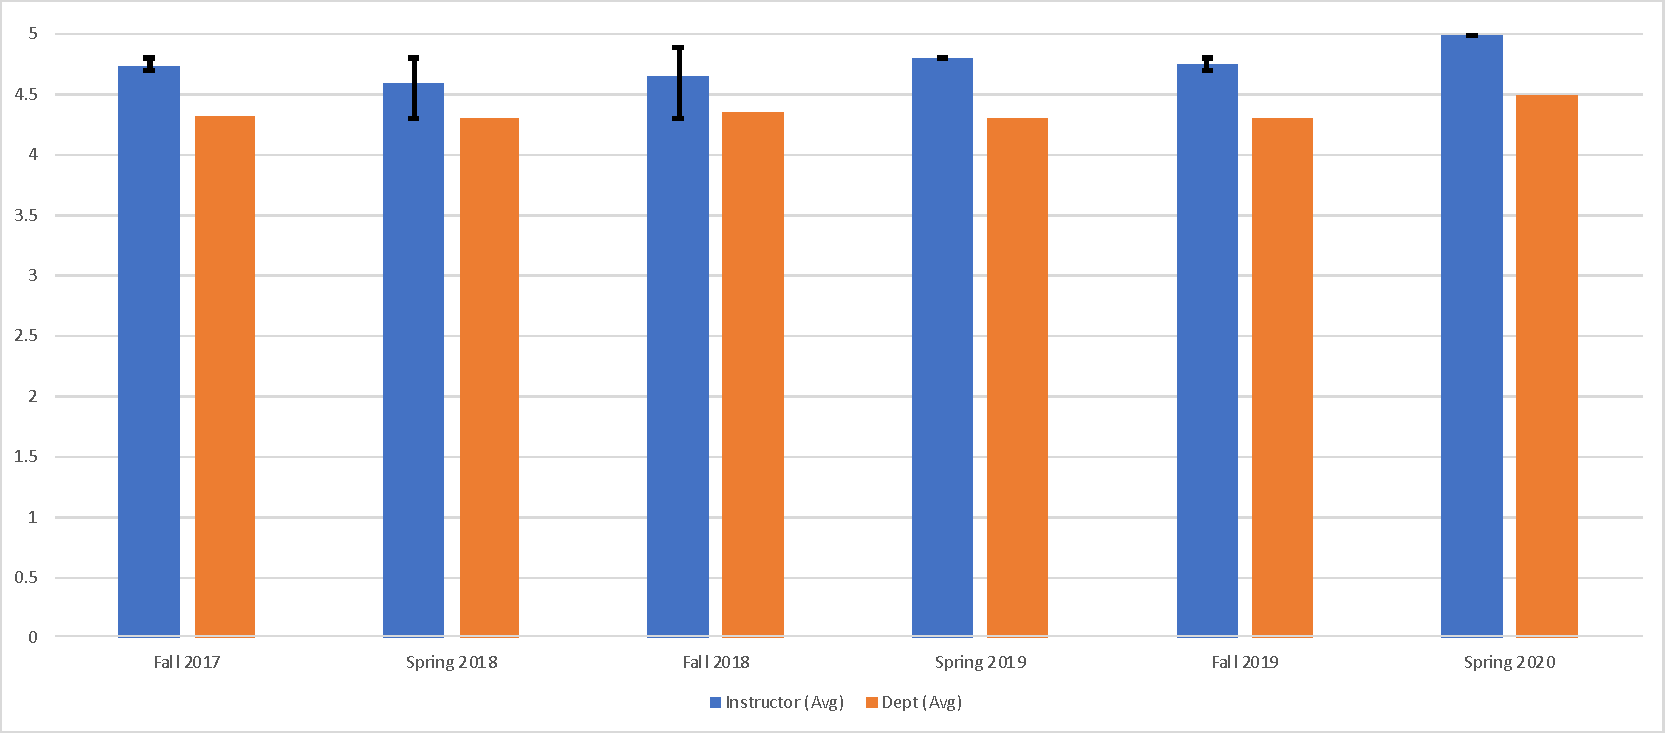
\includegraphics[width=0.9\linewidth]{section-e/files/TRACEChart.pdf}}
            \caption{Summary of TRACE Scores}
            \label{trace-summary}
        \end{figure}
    \end{center}
\end{landscape}